%!TEX root = practicum1.tex
Since \autoref{eq:1:lsChance} only holds when the points are general position we sampled them from a Gaussian distribution for both experiments, since the points are then guaranteed to be linearly independent \cite[Chapter~5]{prince2012computer}. In these experiments we have made the number of patterns dependent upon some parameter $\alpha$ according to: 
	\begin{equation}\label{eq:alpha}
		N = \alpha d.
	\end{equation}
We define $Q_{l.s.}$ as the fraction of data sets where the perceptron found a hyperplane to separate the two classes within the $d_{max}$ epochs.	

\subsection*{Experiment I}
For the first experiment we have sampled 500 50-dimensional from a standard normal distribution. The number of data points per data set is dependent upon \eqref{eq:alpha}, $d_{max}$ was set to 1000. The ratio $Q_{l.s.}$ for different values of $\alpha$ is plotted in \autoref{fig:experiment1:plot}.

\begin{figure}[H]
	\centering
	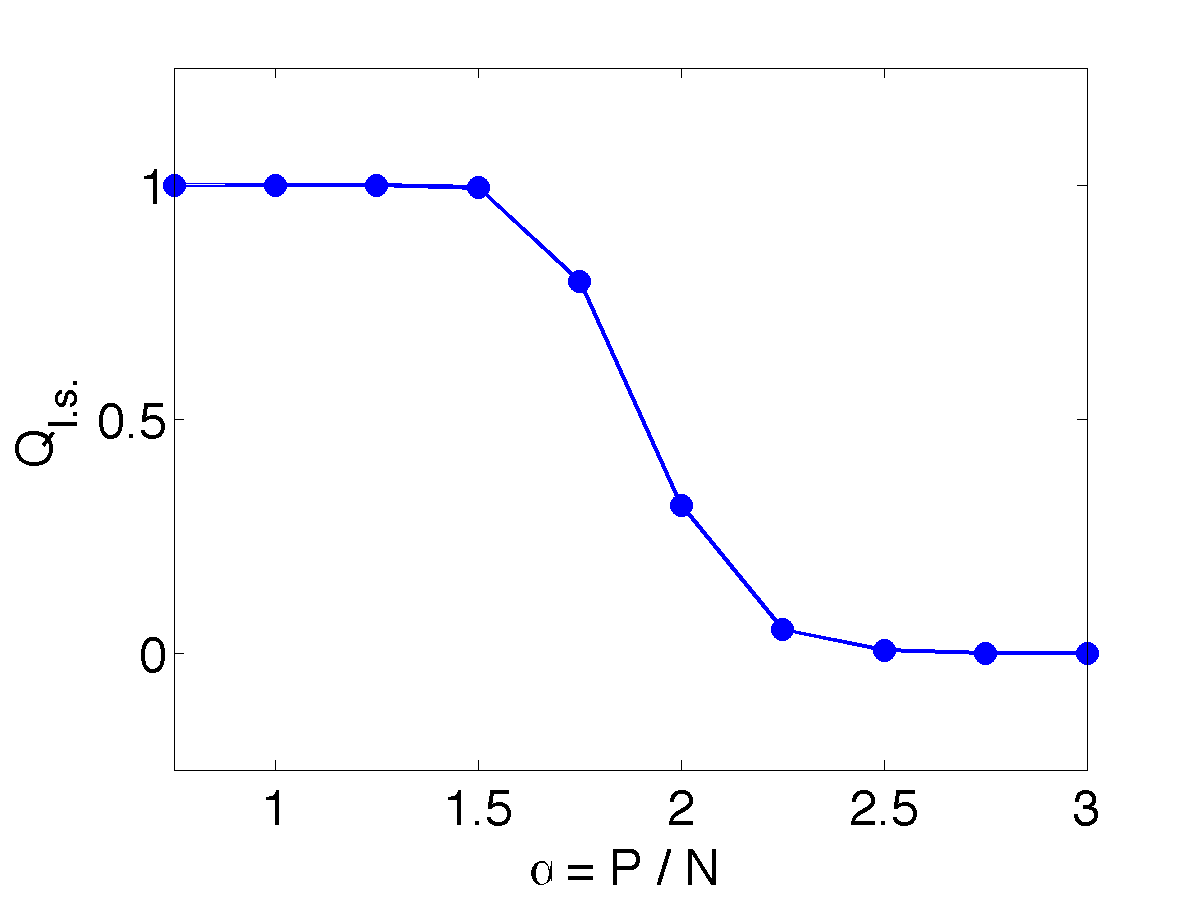
\includegraphics[width=\columnwidth]{./img/Aa_N50_nd500_nmax1000}
	\caption{The parameter $\alpha$ versus $Q_{l.s.}$.}
	\label{fig:experiment1:plot}
\end{figure}

\Cref{fig:experiment1:plot} shows that while $\alpha = 1$ $Q_{l.s.}$ is also one, \todo{Why is this correct}. 

\todo[inline]{Resultaat experiment beschrijven}
\todo[inline]{Waarom wijkt het resultaat van het experiment af van de theorie}

\subsection*{Experiment II}

\todo[inline]{Wat gaan we testen?}
\todo[inline]{Hoe gaan we het testen?}
\todo[inline]{Wat zijn onze onze resultaten}
\todo[inline]{In hoeverre kloppen de resultaten?}